\section{Provided Kinetic Data Structures}
\label{sec:provided_kdss}

Along with the framework, we provide several already implemented kinetic data structures. They currently are 
\begin{description}
\item[\ccc{Kinetic::Sort<Traits, Visitor>}] maintain a list of points
sorted by x-coordinate.
\item[\ccc{Kinetic::Delaunay_triangulation_2<Traits, Visitor,
    Triangulation>}] maintain the Delaunay triangulation of a set of
  two dimensional points
\item[\ccc{Kinetic::Delaunay_triangulation_3<Traits,Visitor,
    Triangulation>}] maintain the Delaunay triangulation of a set of
  three dimensional points.
\item[\ccc{Kinetic::Regular_triangulation_3<Traits, Visitor,
Triangulation}>] maintain the regular triangulation of a set of waiting
three dimensional points.
\item[\ccc{Kinetic::Enclosing_box_2<Traits>},
  \ccc{Kinetic::Enclosing_box_3<Traits>}] restrict points to stay
  within a box by bouncing them off the walls.
\end{description}


\subsection{Two Dimensional Delaunay}
\label{sec:sort_example}

Using a kinetic data structure can be as simple as the following:
\label{fig:sort_program}
\ccIncludeExampleCode{Kinetic_data_structures/sort.C}

In the example, first the Kinetic::SimulationTraits object is chosen
(in this case one that supports exact computations). Then the kinetic
data structure is defined, using the chosen traits object and a
visitor class which logs changes to the sorted list.  Next, instances
of the two are created and a set of points is read from a file. Then,
the simulator is instructed to process all the events until the end of
the simulation.  Finally, a record of what happened is printed to the
terminal.

Several important things happen behind the scenes in this example.
First, the Kinetic::ActiveObjectsTable which holds the moving points
notifies the kinetic data structure that new points have been added to
the simulation. Second, the \ccc{Kinetic::Sort<Traits,Visitor>} kinetic data structure
registers its events with the Kinetic::Simulator by providing a time
and a proxy object. When a particular event occurs, the
Kinetic::Simulator calls a function on the proxy object which in turn
updates the kinetic data structure.

The example illustrates how to monitor the supplied data structures as
they evolve by using a Kinetic::SortVisitor object---a small class whose
methods are called whenever the kinetic data structure changes. Hooks
for such visitor concepts are provided for all of the shipped kinetic
data structures. In the case of kinetic sorting, the visitor's
methods are called every time a new point is inserted in the sorted
list, when one is removed, or when two points are swapped in the
sorted order. 


The visitor concept is quite powerful, allowing us, for example, to
implement a data structure for computing and storing two-dimensional
arrangements of $x$-monotone curves on top of the
\ccc{Kinetic::Sort<Traits, Visitor>} data structure using about 60
lines of code. This sweepline code is presented in
Section~\ref{sec:sweepline_example}.




\subsection{Visualization of Kinetic Data Structures\label{sec:kds_delaunay_2_example}}


The framework includes Qt widgets for displaying kinetic data
structures in two and three dimensions. The following example shows
using the two dimensional widget with a Delaunay triangulation:

\begin{ccExampleCode}
#include <CGAL/Kinetic/Exact_simulation_traits.h>
#include <CGAL/Kinetic/Delaunay_triangulation_2.h>
#include <CGAL/Kinetic/Enclosing_box_2.h>
#include <CGAL/Kinetic/IO/Qt_moving_points_2.h>
#include <CGAL/Kinetic/IO/Qt_triangulation_2.h>
#include <CGAL/Kinetic/IO/Qt_widget_2.h>

int main(int argc, char *argv[]) {
    using namespace CGAL::Kinetic;
    typedef Exact_simulation_traits Traits;
    typedef Delaunay_triangulation_2<Traits> Del_2;
    typedef Enclosing_box_2<Traits> Box_2;
    typedef Qt_widget_2<Traits::Simulator> Qt_widget;
    typedef Qt_moving_points_2<Traits, Qt_gui> Qt_mps;
    typedef Qt_triangulation_2<Del_2, Qt_widget, Qt_mps> Qt_dt2;
    
    // create a simulation traits and add two KDSs:
    // a kinetic Delaunay triangulation and an enclosing box;
    // the moving points bounce against the walls of the enclosing box
    Traits tr;
    Box_2::Handle box = new Box_2(tr);
    Del_2::Handle kdel = new Del_2(tr);

    // register the simulator, set of moving points and
    // Delaunay triangulation with the kinetic Qt widget
    Qt_widget::Handle qt_w = new Qt_widget(argc, argv, tr.simulator_handle());
    Qt_mps::Handle qt_mps = new Qt_mps(qt_w, tr);
    Qt_dt2::Handle qt_dt2 = new Qt_dt2(kdel, qt_w, qt_mps);

    // read the trajectories of the moving points
    //  the simulation traits automatically inserts them in the two KDSs
    // and schedules the appropriate kinetic events; as in the kinetic
    // sorting example this is done with appropriate notifications
    std::ifstream in("data/points_2");    
    in  >> *tr.active_points_2_table_handle();

    // run the interactive kinetic simulation
    return qt_w->begin_event_loop();
};
\end{ccExampleCode}

The example shows how to use a number of additional features of the
framework. First, it shows that two kinetic data structures
(\ccc{Kinetic::Delaunay_triangulation_2<Traits, Triangulation>} and
\ccc{Kinetic::Enclosing_box_2<Traits>}) can coexist on the same set of
points without any extra effort. Both interact with the moving points
through the active objects table, and never need to directly interact
with one another. Second, objects (like
\texttt{qt\_w}, \texttt{qt\_mps} and \texttt{qt\_dt2}) are all stored
by using reference counted handles (\texttt{Object::Handle}). This
allows them to share references to one another without the user having
to worry about memory management and order of deletion.  For example,
the \ccc{Kinetic::Qt_triangulation_2<KineticDelaunay_2, QtWidget_2,
Qt_moving_points_2>} object needs a handle to the kinetic
triangulation, in order to get the structure to display, and a handle
to the \ccc{Active_points_1_table} to get the coordinates of the
points.


Finally, the example shows how to use the graphical interface elements
provided, see Figure~\ref{fig:kds_qtwidget_capture}. Our package includes
\texttt{Qt} widgets for displaying kinetic geometry in two and three
dimensions. In addition to being able to play and pause the
simulation, the user can step through events one at a time and reverse
the simulation to retrace what had happened. The three-dimensional
visualization support is based on the Coin library http://www.coin3d.org.

\begin{figure*}[htb]
\begin{ccTexOnly}
\begin{center}
1.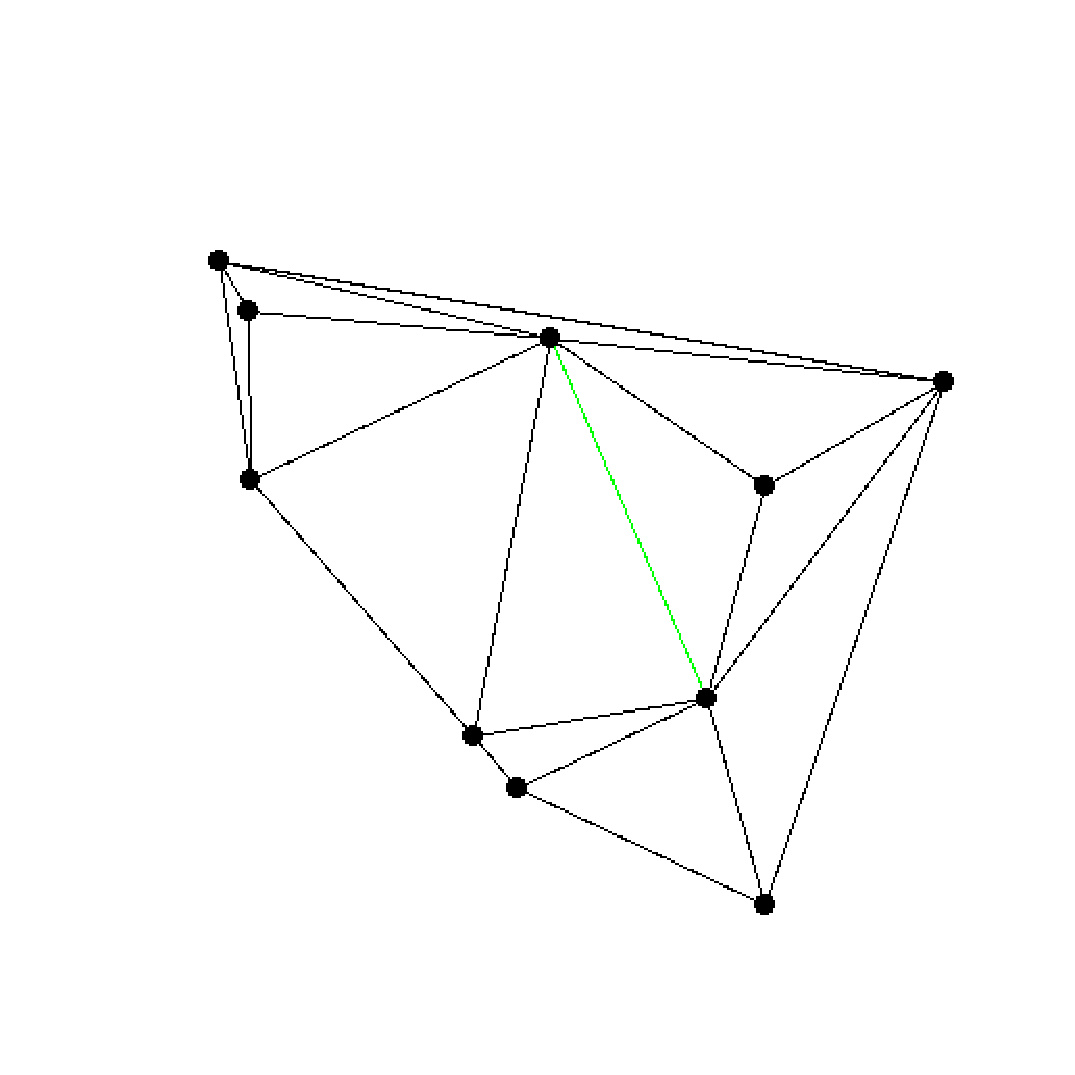
\includegraphics[ scale=.2]{Kinetic_data_structures/delaunay_0} 
2.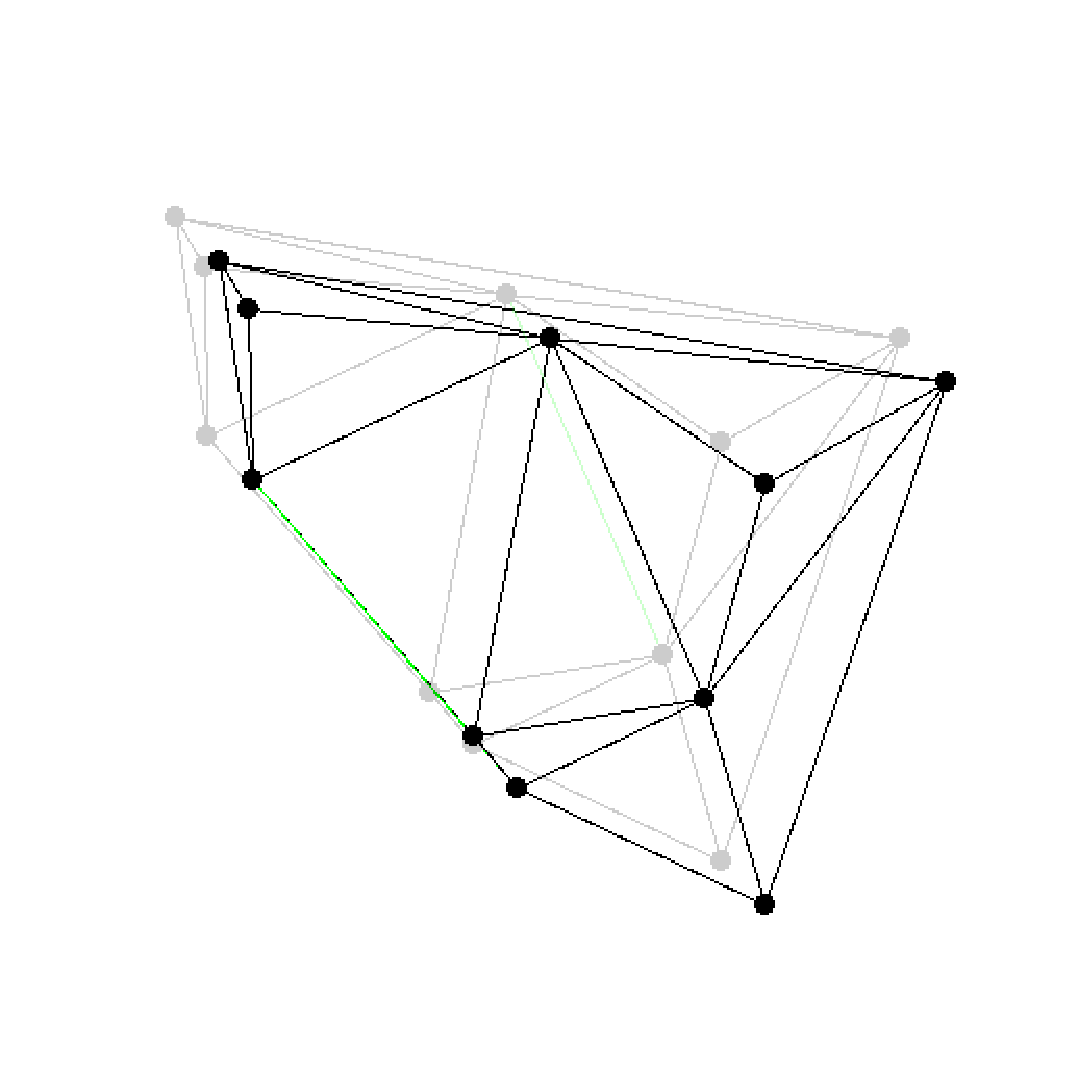
\includegraphics[ scale=.2]{Kinetic_data_structures/delaunay_1}
3.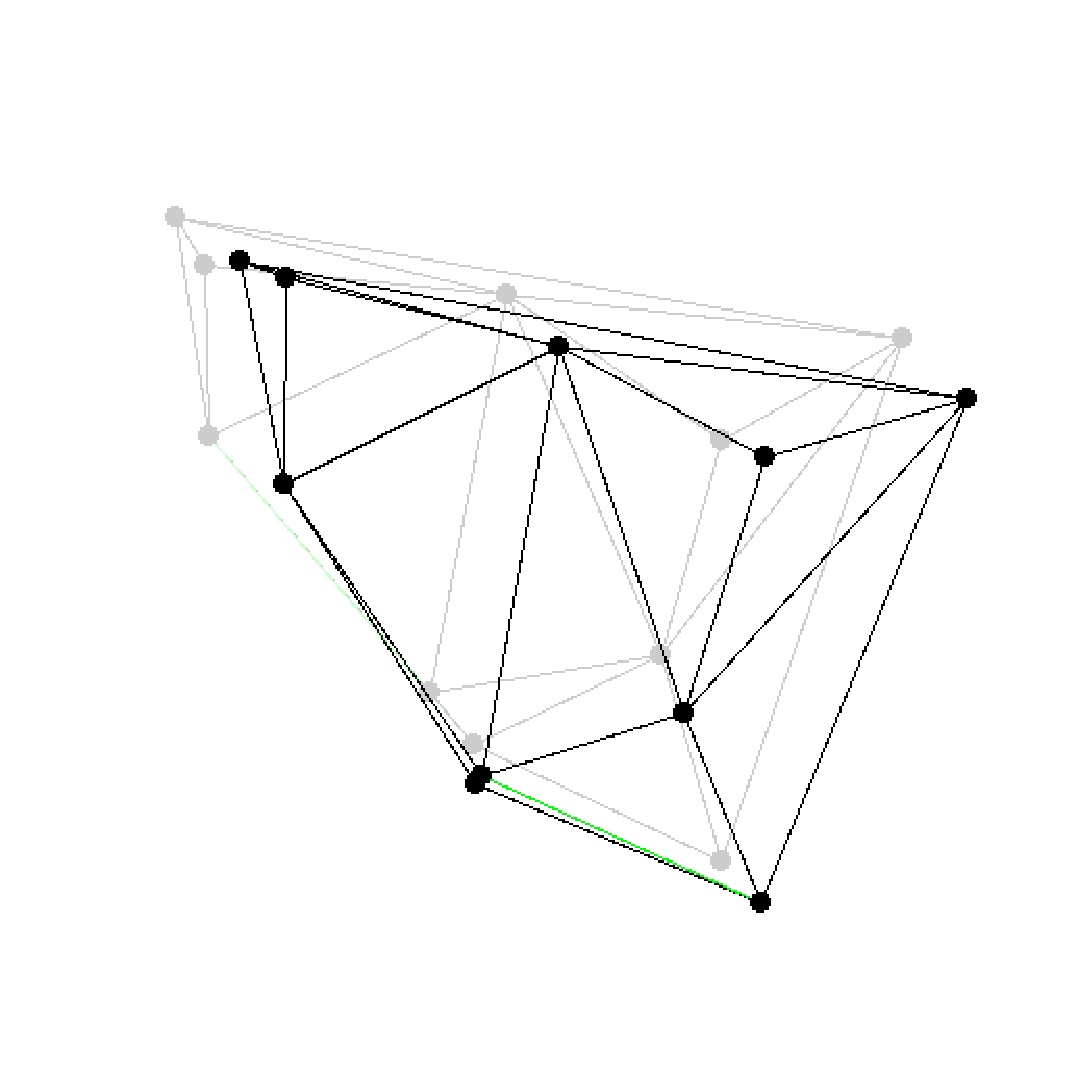
\includegraphics[ scale=.2]{Kinetic_data_structures/delaunay_2}\\
4.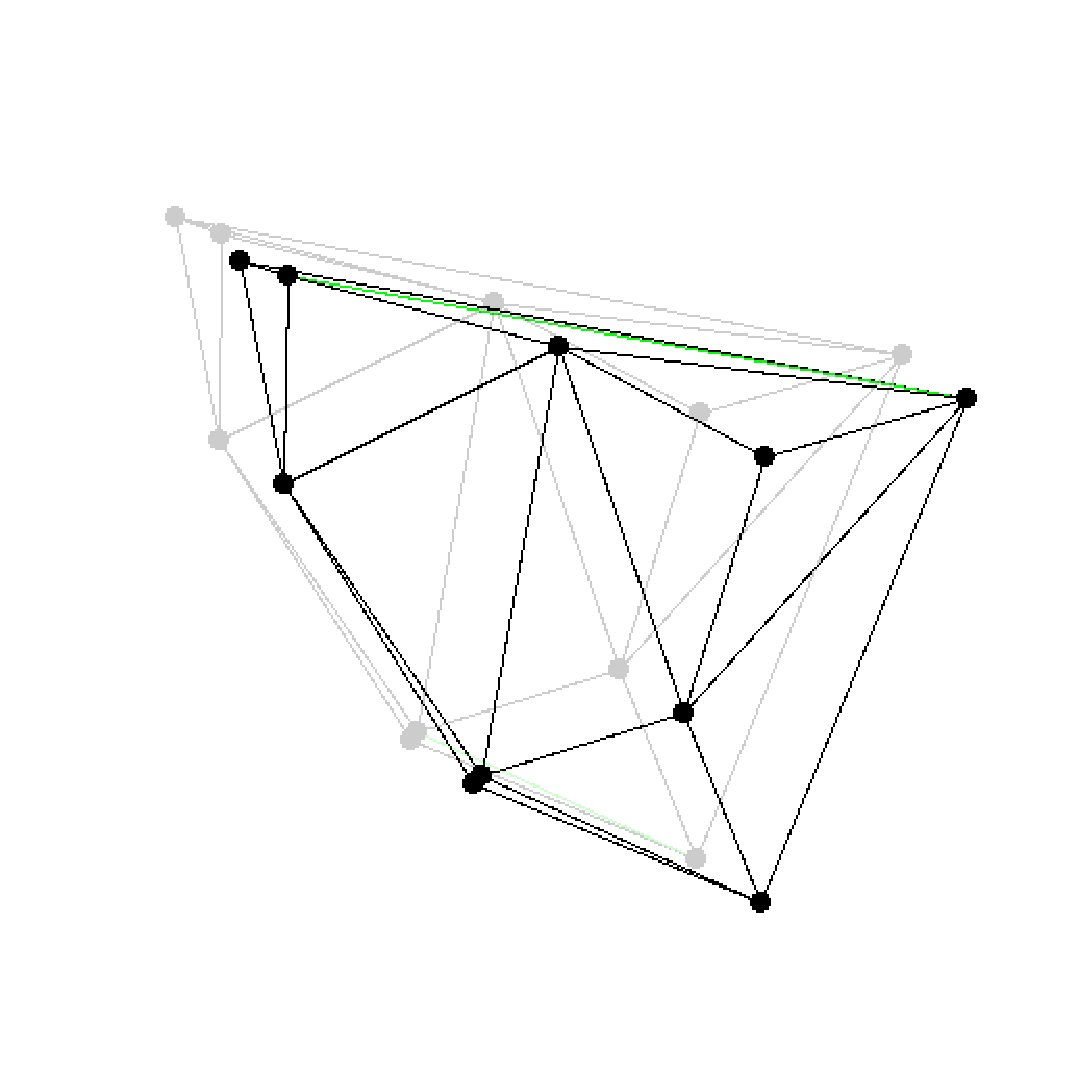
\includegraphics[ scale=.2]{Kinetic_data_structures/delaunay_3}
5.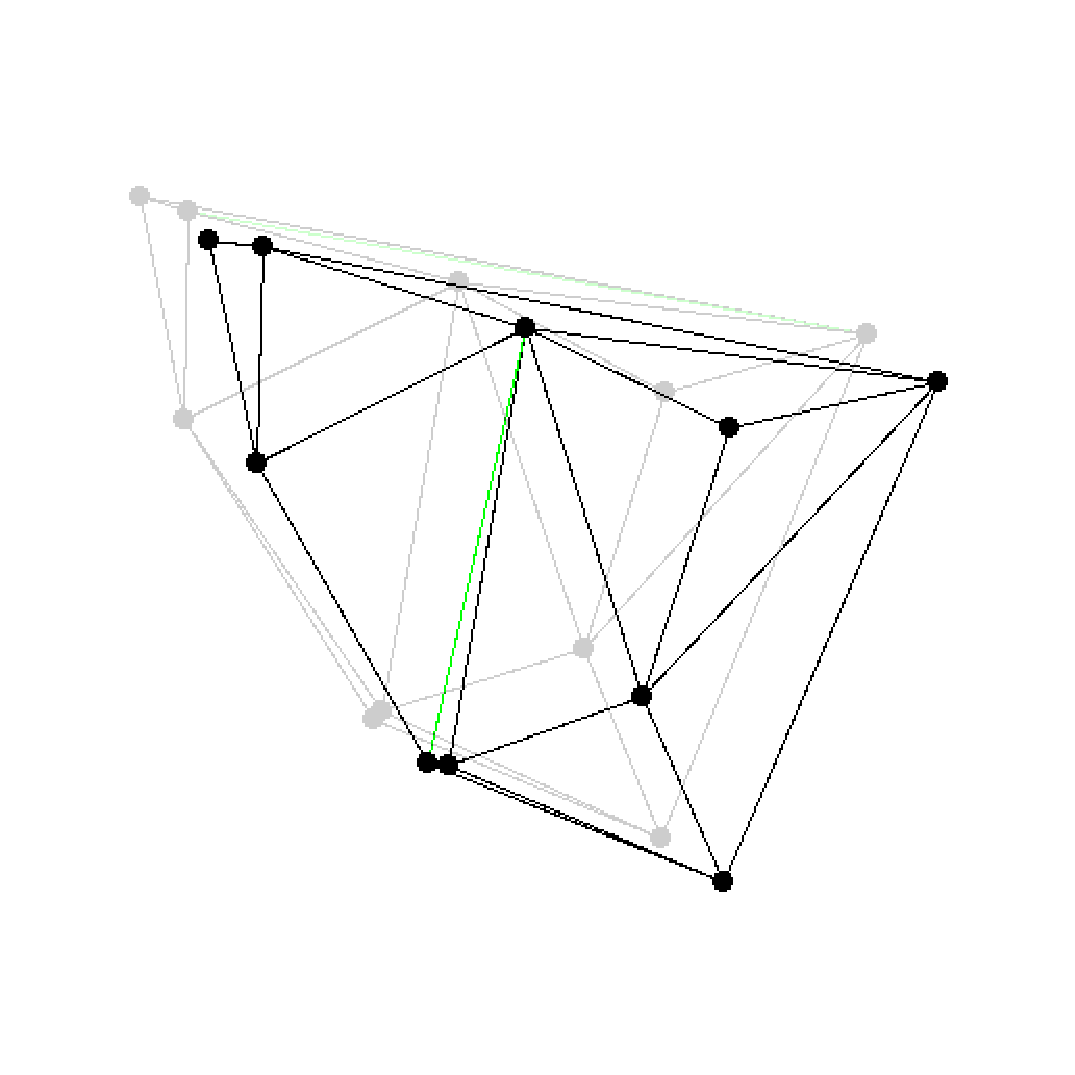
\includegraphics[ scale=.2]{Kinetic_data_structures/delaunay_4}
6.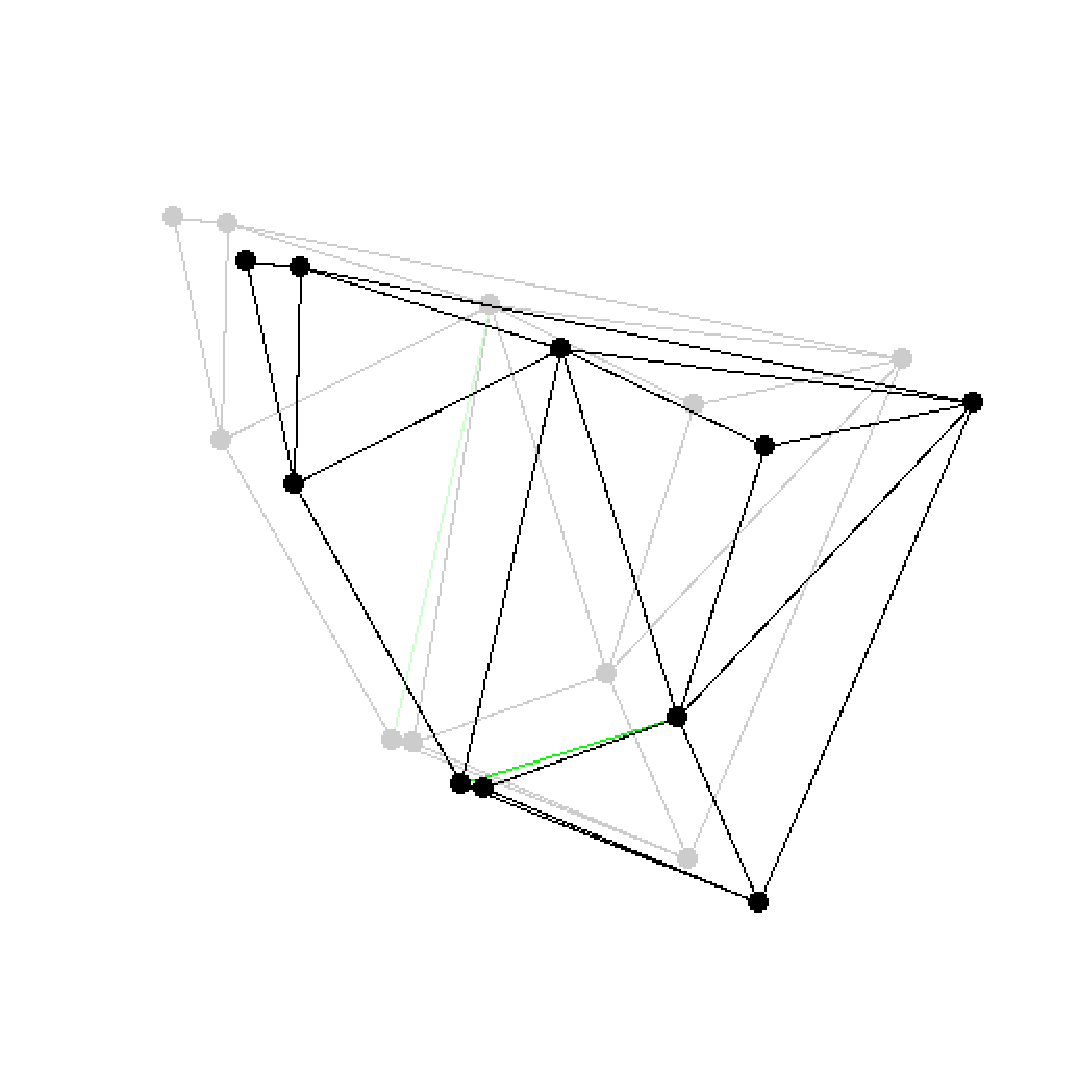
\includegraphics[ scale=.2]{Kinetic_data_structures/delaunay_5}\\
7.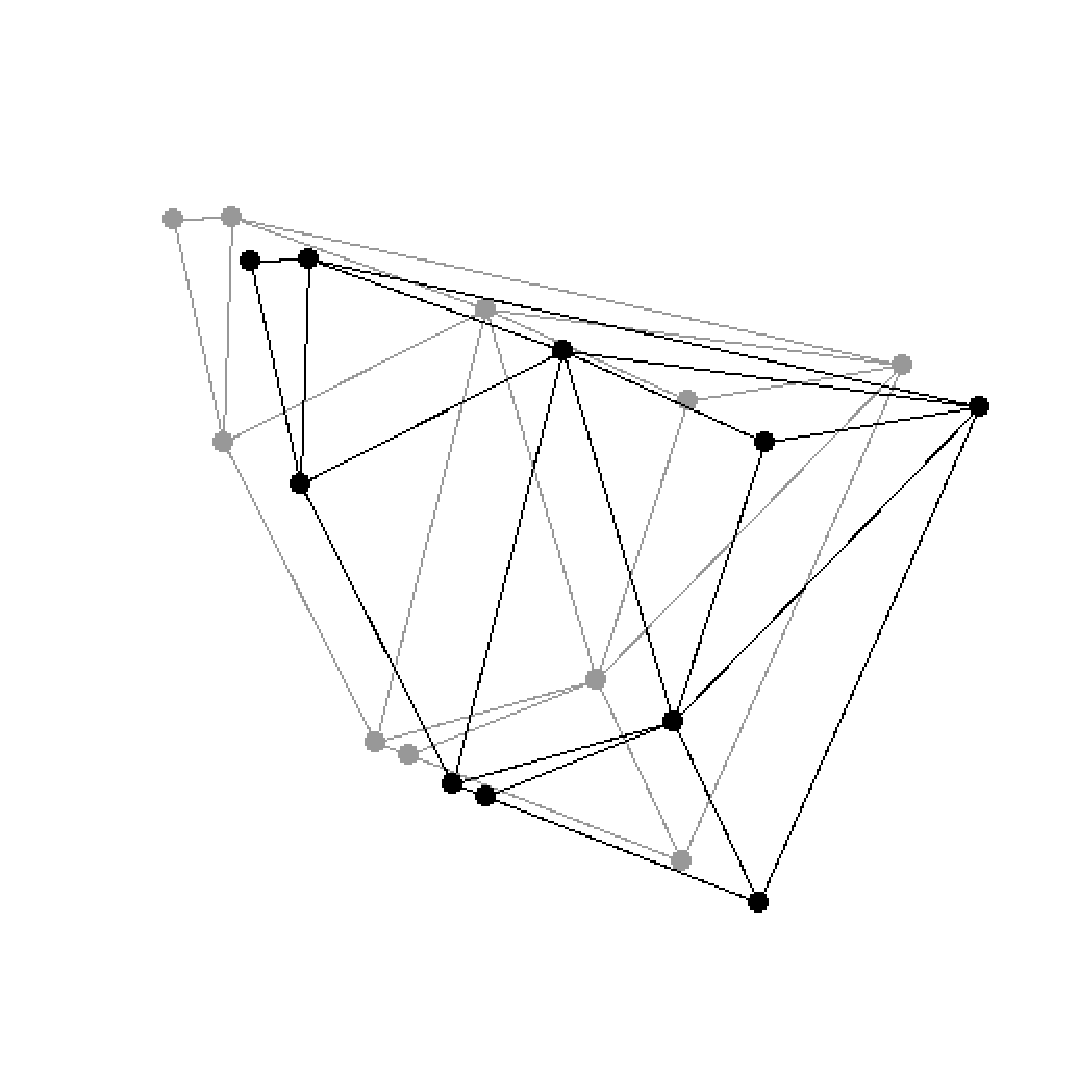
\includegraphics[ scale=.2]{Kinetic_data_structures/delaunay_6}
8.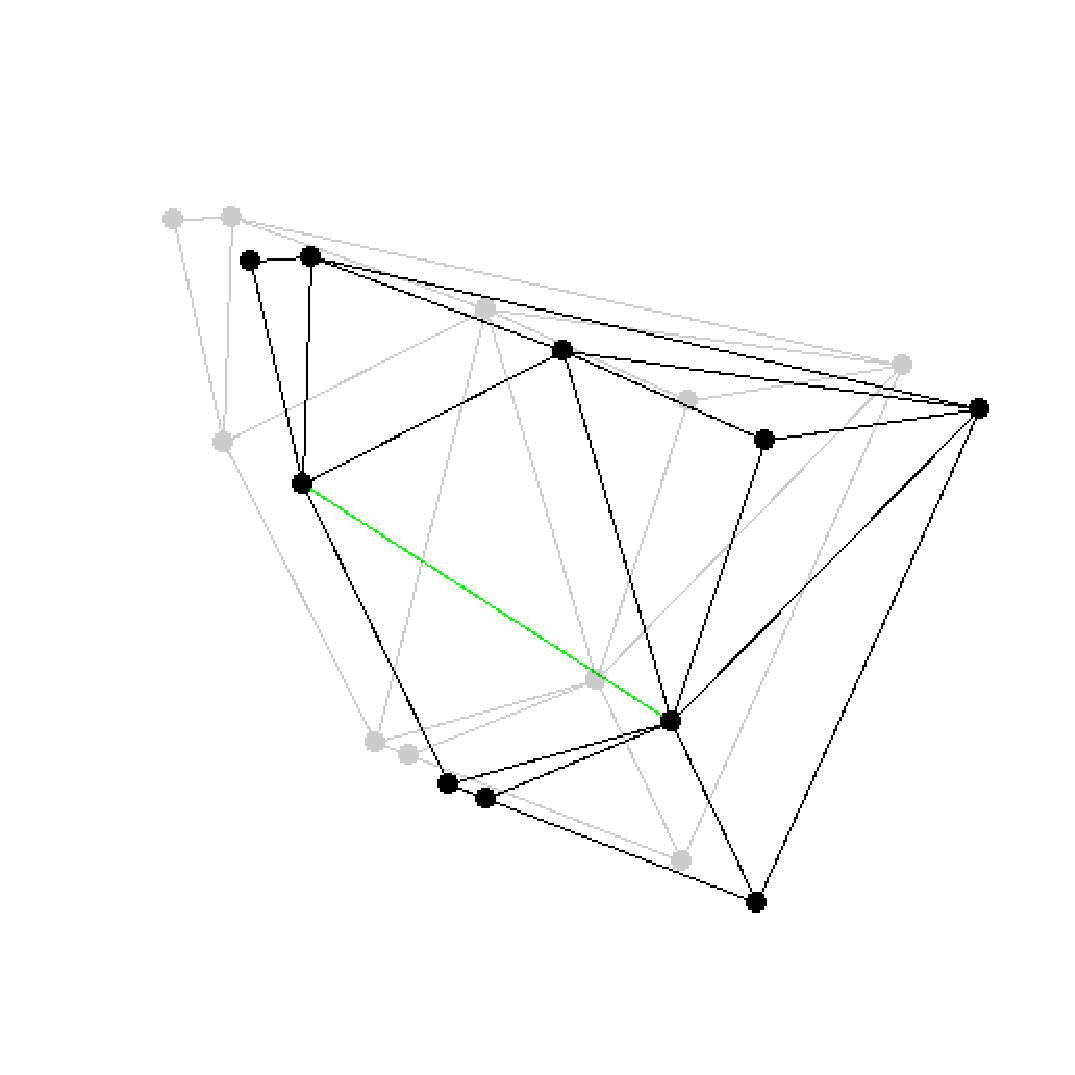
\includegraphics[ scale=.2]{Kinetic_data_structures/delaunay_7}
9.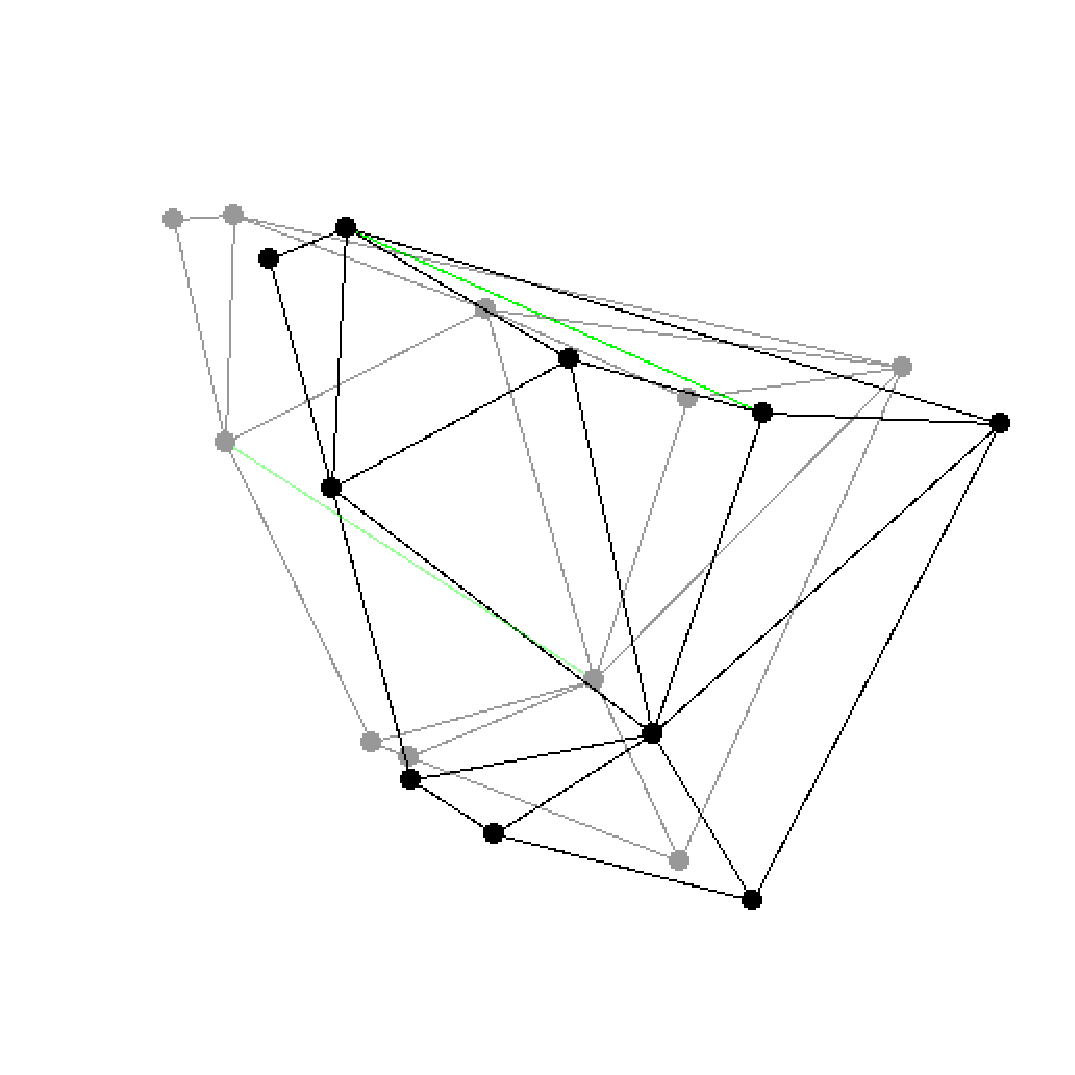
\includegraphics[ scale=.2]{Kinetic_data_structures/delaunay_8}
\end{center}
\end{ccTexOnly}
%width=300 height=300
\begin{ccHtmlOnly}

<img border=1 src="./delaunay_0.gif" align=middle alt="Frame 0" >
<img border=1 src="./delaunay_1.gif" align=middle alt="Frame 1" >
<img border=1 src="./delaunay_2.gif" align=middle alt="Frame 2" >
<img border=1 src="./delaunay_3.gif" align=middle alt="Frame 3" >
<img border=1 src="./delaunay_4.gif" align=middle alt="Frame 4" >
<img border=1 src="./delaunay_5.gif" align=middle alt="Frame 5" >
<img border=1 src="./delaunay_6.gif" align=middle alt="Frame 6" >
<img border=1 src="./delaunay_7.gif" align=middle alt="Frame 7" >
<img border=1 src="./delaunay_8.gif" align=middle alt="Frame 8" >
<br>
\end{ccHtmlOnly}
\caption{ \label{fig:kds_delaunay_events} 
{\em Some events from a Delaunay triangulation kinetic data
structure:} The state of the two dimensional Delaunay triangulation
immediately following the first events is shown. Green edges are ones
which were just created. The pictures are screen shots from
\ccc{demo/Kinetic\_data\_structures/Kinetic\_Delaunay\_triangulation\_2.cpp}. }
%\end{minipage}
%\end{center}
\end{figure*}


\begin{figure}
\begin{ccTexOnly}
\begin{center}
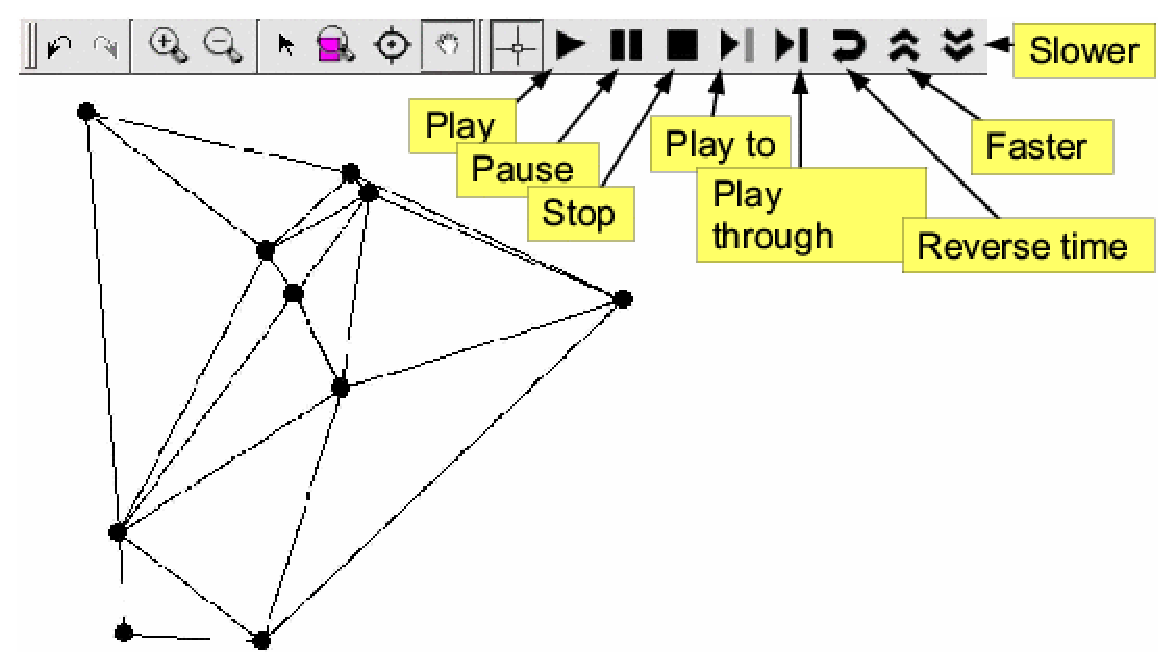
\includegraphics[scale=.5]{Kinetic_data_structures/qt_widget_marked_pct}
\end{center}
\end{ccTexOnly}
\begin{ccHtmlOnly}
<img src="./qt_widget_marked_pct.gif" align=middle alt="Qt widget"> <br>
\end{ccHtmlOnly}
\caption{\label{fig:kds_qtwidget_capture} The figure shows the graphical user interface for
  controlling two-dimensional kinetic data structures. It is built on
  top of the \ccc{Qt_widget} and adds buttons to play, pause, step
  through and run the simulation backwards.}
\end{figure}



%%% Local Variables: 
%%% mode: latex
%%% TeX-master: t
%%% End: 
